\documentclass[tikz,border=4pt]{standalone}
\usepackage[T1]{fontenc}
\usepackage{lmodern}
\usepackage{amsmath,amssymb}
\input{four_routes_values}
\usetikzlibrary{arrows.meta,positioning}
\begin{document}
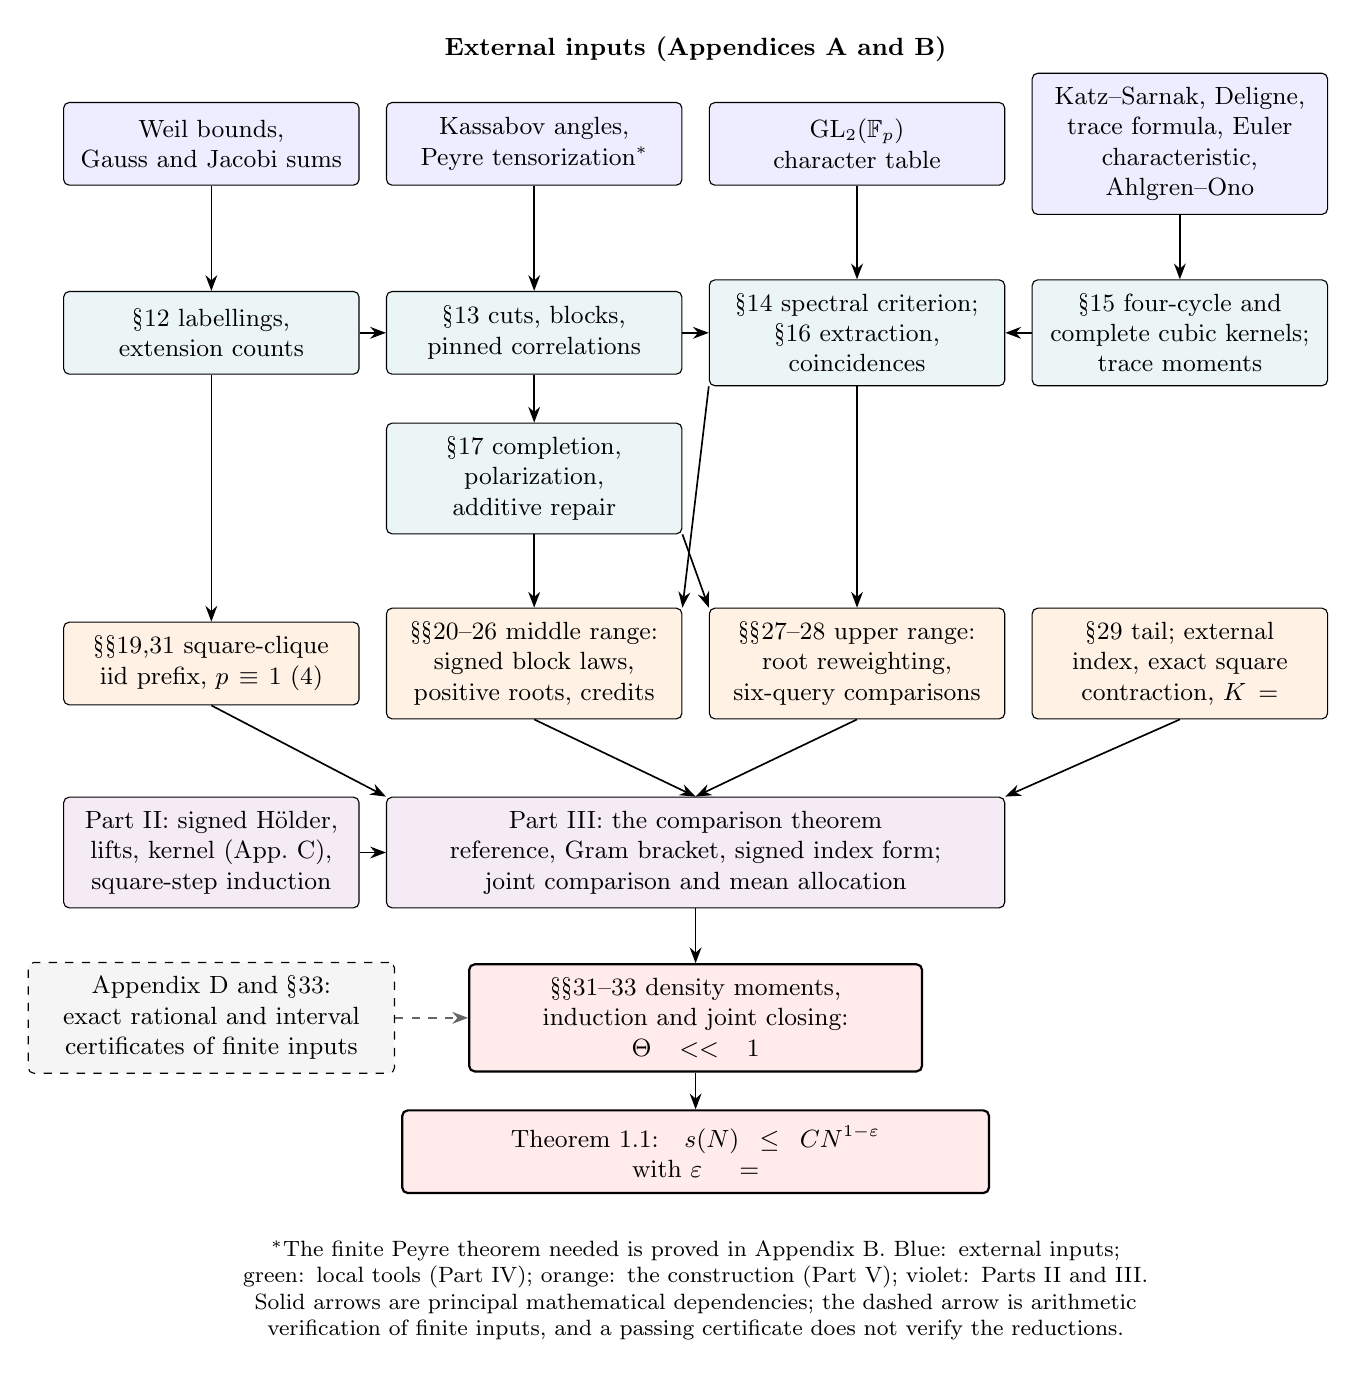
\begin{tikzpicture}[
 box/.style={draw,rounded corners=2pt,align=center,inner sep=5pt,execute at begin node={\hyphenpenalty=10000\exhyphenpenalty=10000},
  text width=3.4cm,minimum height=1.05cm,font=\small},
 ext/.style={box,fill=blue!7},
 tool/.style={box,fill=teal!8},
 law/.style={box,fill=orange!10},
 frame/.style={box,fill=violet!8},
 result/.style={box,fill=red!8,text width=7.1cm,thick},
 check/.style={box,fill=gray!8,dashed,text width=6.0cm},
 arr/.style={-{Stealth[length=2mm]},semithick},
 checked/.style={arr,dashed,gray!80!black},
 heading/.style={font=\small\bfseries,align=center}
]
\node[heading] at (6.15,1.2) {External inputs (Appendices A and B)};
\node[ext] (weil) at (0,0) {Weil bounds,\\Gauss and Jacobi sums};
\node[ext] (angle) at (4.1,0) {Kassabov angles,\\Peyre tensorization$^*$};
\node[ext] (group) at (8.2,0) {$\mathrm{GL}_2(\mathbb F_p)$\\character table};
\node[ext] (geometry) at (12.3,0) {Katz--Sarnak, Deligne,\\trace formula, Euler\\characteristic,\\Ahlgren--Ono};
\node[tool] (counts) at (0,-2.4) {\S12 labellings,\\extension counts};
\node[tool] (corr) at (4.1,-2.4) {\S13 cuts, blocks,\\pinned correlations};
\node[tool] (spec) at (8.2,-2.4) {\S14 spectral criterion;\\\S16 extraction,\\coincidences};
\node[tool] (second) at (12.3,-2.4) {\S15 four-cycle and\\complete cubic kernels;\\trace moments};
\node[tool] (completion) at (4.1,-4.25) {\S17 completion,\\polarization,\\additive repair};
\draw[arr] (weil) -- (counts);
\draw[arr] (angle) -- (corr);
\draw[arr] (group) -- (spec);
\draw[arr] (geometry) -- (second);
\draw[arr] (counts) -- (corr);
\draw[arr] (corr) -- (spec);
\draw[arr] (second) -- (spec);
\draw[arr] (corr) -- (completion);
\node[law] (prefix) at (0,-6.6) {\S\S19,31 square-clique\\iid prefix, $p\equiv1\ (4)$};
\node[law] (middle) at (4.1,-6.6) {\S\S20--26 middle range:\\signed block laws,\\positive roots, credits};
\node[law] (upper) at (8.2,-6.6) {\S\S27--28 upper range:\\root reweighting,\\six-query comparisons};
\node[law] (index) at (12.3,-6.6) {\S29 tail; external\\index, exact square\\contraction, $K=\FourRoutesK$};
\draw[arr] (completion.south) -- (middle.north);
\draw[arr] (completion.south east) -- (upper.north west);
\draw[arr] (spec.south) -- (upper.north);
\draw[arr] (spec.south west) -- (middle.north east);
\draw[arr] (counts.south) -- (prefix.north);
\node[frame] (analytic) at (0,-9.0) {Part II: signed H\"older,\\lifts, kernel (App.~C),\\square-step induction};
\node[frame,text width=7.5cm] (comparison) at (6.15,-9.0) {Part III: the comparison theorem\\reference, Gram bracket, signed index form;\\joint comparison and mean allocation};
\draw[arr] (analytic) -- (comparison);
\draw[arr] (prefix.south) -- (comparison.north west);
\draw[arr] (middle.south) -- (comparison.north);
\draw[arr] (upper.south) -- (comparison.north);
\draw[arr] (index.south) -- (comparison.north east);
\node[result,text width=5.4cm] (closing) at (6.15,-11.1) {\S\S31--33 density moments,\\induction and joint closing:\\$\Theta<\FourRoutesTheta<1$};
\draw[arr] (comparison) -- (closing);
\node[result] (theorem) at (6.15,-12.8) {Theorem 1.1:\quad $s(N)\le C N^{1-\varepsilon}$\\with $\varepsilon=\FourRoutesDecimal$};
\draw[arr] (closing) -- (theorem);
\node[check,text width=4.3cm] (finite) at (0,-11.1) {Appendix D and \S33:\\exact rational and interval\\certificates of finite inputs};
\node[box,draw=none,text width=12.5cm,font=\footnotesize,anchor=north] at (6.15,-13.75)
 {$^*$The finite Peyre theorem needed is proved in Appendix~B. Blue: external inputs; green: local tools (Part IV); orange: the construction (Part V); violet: Parts II and III. Solid arrows are principal mathematical dependencies; the dashed arrow is arithmetic verification of finite inputs, and a passing certificate does not verify the reductions.};
\draw[checked] (finite.east) -- (closing.west);
\end{tikzpicture}
\end{document}
